\documentclass[dvipdfmx]{ujarticle}
\usepackage{amsmath,amssymb,amsfonts}
\usepackage{graphicx}
\usepackage[margin=0.7in]{geometry}
\usepackage{ascmac}
\usepackage{subfig}

\begin{document}
\author{Koki Kitamori}
\title{Cubic Spline Function Result}
\西暦
\date{\today}
\maketitle

\section{}
\subsection*{A)}

cubic regression splineでCSVで与えられたデータ点を,以下に記載するじJulia言語によるプログラムで近似した.
赤色の線が各領域での近似曲線を繋ぎ合わせたスプライン関数である.
求める手順を以下に示す.

まず,与えられたデータから行列$X$,ベクトル$\boldsymbol{y}$を作る.$c_k$は$k$番目のknotの位置である.

\begin{equation}
\mathbf{X}=\left(\begin{array}{cccc}
h_{0}\left(x_{1}\right) & h_{1}\left(x_{1}\right) & \cdots & h_{K+3}\left(x_{1}\right) \\
\vdots & \vdots & & \vdots \\
h_{0}\left(x_{k}\right) & h_{1}\left(x_{k}\right) & \cdots & h_{K+3}\left(x_{k}\right) \\
\vdots & \vdots & & \vdots \\
h_{0}\left(x_{n}\right) & h_{1}\left(x_{n}\right) & \cdots & h_{K+3}\left(x_{n}\right)
\end{array}\right), \quad \boldsymbol{y}=\left(\begin{array}{c}
y_{1} \\
\vdots \\
y_{k} \\
\vdots \\
y_{n}
\end{array}\right)
\end{equation}
ここで,$h_{0}(x)=1, h_{1}(x)=x, h_{2}(x)=x^{2}, h_{3}(x)=x^{3}, h_{k+3}(x)=\left(x-c_{k}\right)_{+}^{3}, k=1,2, \ldots, K$である.次に,

\begin{equation}
\hat{\boldsymbol{\beta}}=\left(\mathbf{X}^{T} \mathbf{X}\right)^{-1} \mathbf{X}^{T} \boldsymbol{y}
\end{equation}
により,$\hat{\boldsymbol{\beta}}$を求めることができる.
最後に次の計算をすれば,3次スプライン関数が求まる.

\begin{equation}
f(x)=\hat\beta_{0} h_{0}(x)+\hat\beta_{1} h_{1}(x)+\cdots+\hat\beta_{K+3} h_{K+3}(x)=\sum_{k=0}^{K+3} \hat\beta_{k} h_{k}(x)
\end{equation}

\begin{figure}[htbp]
    \centering
    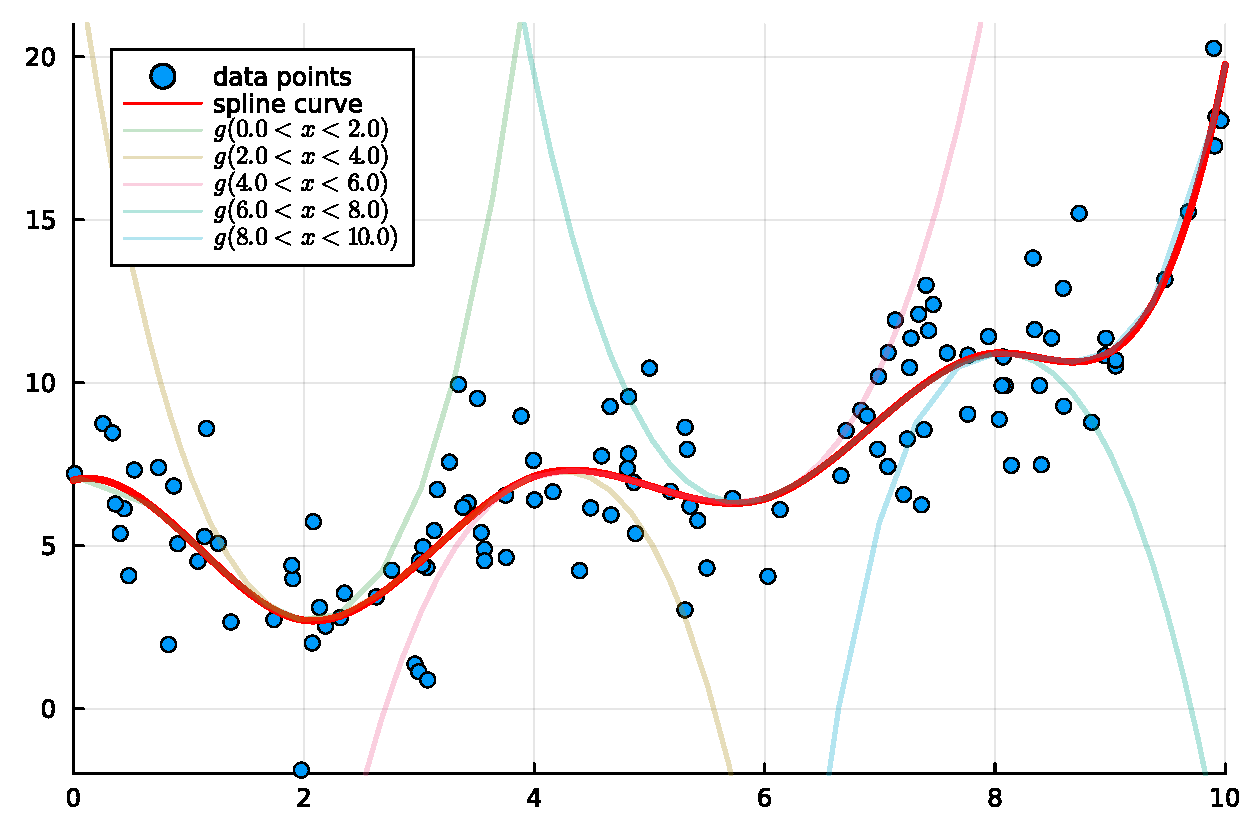
\includegraphics[width=.7\textwidth]{Result/4.pdf}
    \caption{4 knots cubic regression spline}
\end{figure}

\small{
\begin{screen}
\begin{verbatim}
# load library
using CSV, Plots, DataFrames, Polynomials, LinearAlgebra

# define cubic spline function and return x and fitted polynomial function
function cubic_regression_spline(x, y, K, k)
    X = [j ≤ 3 ? x[i]^j : max(0, (x[i] - k[j-3])^3) for i in eachindex(x), j in 0:K+3]
    # calculate linear regression
    β = (X' * X) \ X' * y
    # declare Polynomial array
    g = Polynomial[Polynomial(β[1:4])]
    # calculate spline function for all cases
    for i in 1:K
        push!(g, g[end] + β[i+4] * Polynomial([-k[i]^3, 3k[i]^2, -3k[i], 1]))
    end
    return X, g
end

# define function in otder to plot the spline function
function plot_spline(x, y, K, g, st)
    scatter(x, y, label="data points", legend=:topleft)
    for i in 1:K+1
        i == 1 ? plot!(g[i], label="spline curve", xlims=(st * (i - 1), st * i), c="red", lw=3) :
        plot!(g[i], label="", xlims=(st * (i - 1), st * i), c="red", lw=3)
        plot!(g[i], label="\$g($(round(st * (i - 1), digits=1))<x<$(round(st * i, digits=1)))\$",
            xlims=(0, 10), ylims=(-2, 21), xaxis=0:2:10, alpha=0.3, lw=2)
    end
    savefig("$K.pdf")
end


# ------------------------------------------------------------------------------------------------ #
# load data
data = Matrix(CSV.read("TrainingDataForAssingment5.csv", DataFrame))[:, 2:3]
x, y = data[:, 1], data[:, 2]
scatter(x, y, label="data points", legend=:topleft)

K = 4 # number of knots
k = [2, 4, 6, 8] # knots
X, g = cubic_regression_spline(x, y, K, k)
plot_spline(x, y, K, g, 2)

\end{verbatim}
\end{screen}}\normalsize

\subsection*{B}
A)で示した手順に基づき,プログラムを作成・実行することにより求めた$f(x)$は次のようになった.
cubic regression splineとその関数の描画は今回のレポートで実行する回数が非常に多いため関数化し,cubic\_regression\_spline, plot\_splineという2つの関数を作成している.
cubic\_regression\_splineにより,行列$\mathbf{X}$と$\hat{\boldsymbol{\beta}}$を求めスプライン関数での回帰を行った.

\begin{equation}
f(x)=\left\{\begin{array}{l}
7.008+0.946 x-3.912 x^{2}+1.183 x^{3} \quad (0\le x \le 2) \\
23.783-24.217 x+8.669 x^{2}-0.914 x^{3} \quad (2\le x \le 4) \\
-82.527+55.516 x-11.264 x^{2}+0.747 x^{3} \quad (4\le x \le 6) \\
249.853-110.674 x+16.434 x^{2}-0.792 x^{3} \quad (6\le x \le 8) \\
-1344.032+487.032 x-58.280 x^{2}+2.321 x^{3} \quad (8\le x \le 10) \\
0 \quad (otherwise)
\end{array}\right.
\end{equation}

\small{
\begin{screen}
\begin{verbatim}
# C) Leave on out cross validation using hat matrix (magic foemula)
function calc_CVLOO_magic(X, x, g, y, st)
    diag_H = diag(X * ((X' * X) \ X'))
    f = [g[Int(ceil(i / st))](i) for i in x]
    CV_LOO = sum([((y[i] - f[i]) / (1 - diag_H[i]))^2 for i in 1:length(y)]) / length(y)
    println(CV_LOO)
end
calc_CVLOO_magic(X, x, g, y, 2)

# ------------------------------------------------------------------------------------------------ #
# D) Leave on out cross validation without magic formula
CV_LOO_2 = 0.0
for iter in 1:length(y)
    # remove the first element of x and y
    x_, y_ = popfirst!(x), popfirst!(y)
    # fit by cubic spline function
    local X, g = cubic_regression_spline(x, y, K, k)
    # calculate CVLOO for each element
    global CV_LOO_2 += (y_ - g[Int(ceil(x_ / 2))](x_))^2
    # append x_ and y_ as the last element of x and y respectively
    push!(x, x_)
    push!(y, y_)
end
println(CV_LOO_2 / length(y))

# ------------------------------------------------------------------------------------------------ #
# use CVLOO to determine the number of knots among 1,2,...,15
for K_ in 1:15
    # calculate uniform knots
    k_ = [10i / (K_ + 1) for i in 1:K_]
    # calculate distance between 2 konts
    st = 10 / (K_ + 1)
    local X, g = cubic_regression_spline(x, y, K_, k_)
    plot_spline(x, y, K_, g, st)
    calc_CVLOO_magic(X, x, g, y, st)
end
\end{verbatim}
\end{screen}}

\subsection*{C}
次式magic formulaを用いて$\mathrm{CV}_{\mathrm{LOO}}$を求めた.
\begin{equation}
\mathrm{CV}_{\mathrm{LOO}}=\frac{1}{n} \sum_{i=1}^{n}\left\{\frac{y_{i}-\hat{f}{\left(x_{i}\right)}}{\left(1-h_{i i}\right)}\right\}^{2} \tag{magic formula}
\end{equation}
\begin{equation}
\text{where} h_{i i} \text { is the } i \text { th diagonal element of } \mathbf{H}=\mathbf{X}\left(\mathbf{X}^{T} \mathbf{X}\right)^{-1} \mathbf{X}^{T}
\end{equation}

プログラムではまず,対角成分を計算しそれを配列化している.
そして,与えられたデータ点に対して予測値を求めている.
最後にmagic formulaを用いて計算している.

以上の手順で求めた結果,\underline{$\mathrm{CV}_{\mathrm{LOO}}=3.7273$}となった.

\subsection*{D}

\begin{enumerate}
  \item ベクトル$\boldsymbol{x}$とベクトル$\boldsymbol{y}$の先頭要素を取り除き,$x\_, y\_$という変数にそれぞれ格納しておく.
  \item cubic\_regression\_spline関数を実行し,取り除いた要素に対して$\left(y_{i}-\hat{f}_{-i}\left(x_{i}\right)\right)^{2}$を求める.
  \item それをすべてのデータ点について繰り返す.
  \item 誤差平方和を求め,要素数で割る.
\end{enumerate}

以上の手順で求めた結果,\underline{$\mathrm{CV}_{\mathrm{LOO}}=3.7273$}となった.

\clearpage
\section{}
$K=1,...,15$としたときの$\mathrm{CV_{LOO}}$の値は次の表のように変化した.
また,その変化の様子を次の図2に示した.

\begin{table}[htbp]
\centering
\resizebox{\textwidth}{!}{%
\begin{tabular}{c||ccccccccccccccc}
$K$ & 1 & 2 & 3 & 4 & 5 & 6 & 7 & 8 & 9 & 10 & 11 & 12 & 13 & 14 & 15 \\ \hline
$\mathrm{CV_{LOO}}$ & 4.375 & 4.366 & 4.411 & 3.727 & 3.959 & 3.789 & 3.844 & 4.152 & 4.392 & 4.649 & 4.688 & 5.269 & 5.767 & 6.121 & 5.927
\end{tabular}%
}
\end{table}

\begin{figure}[htbp]
    \centering
    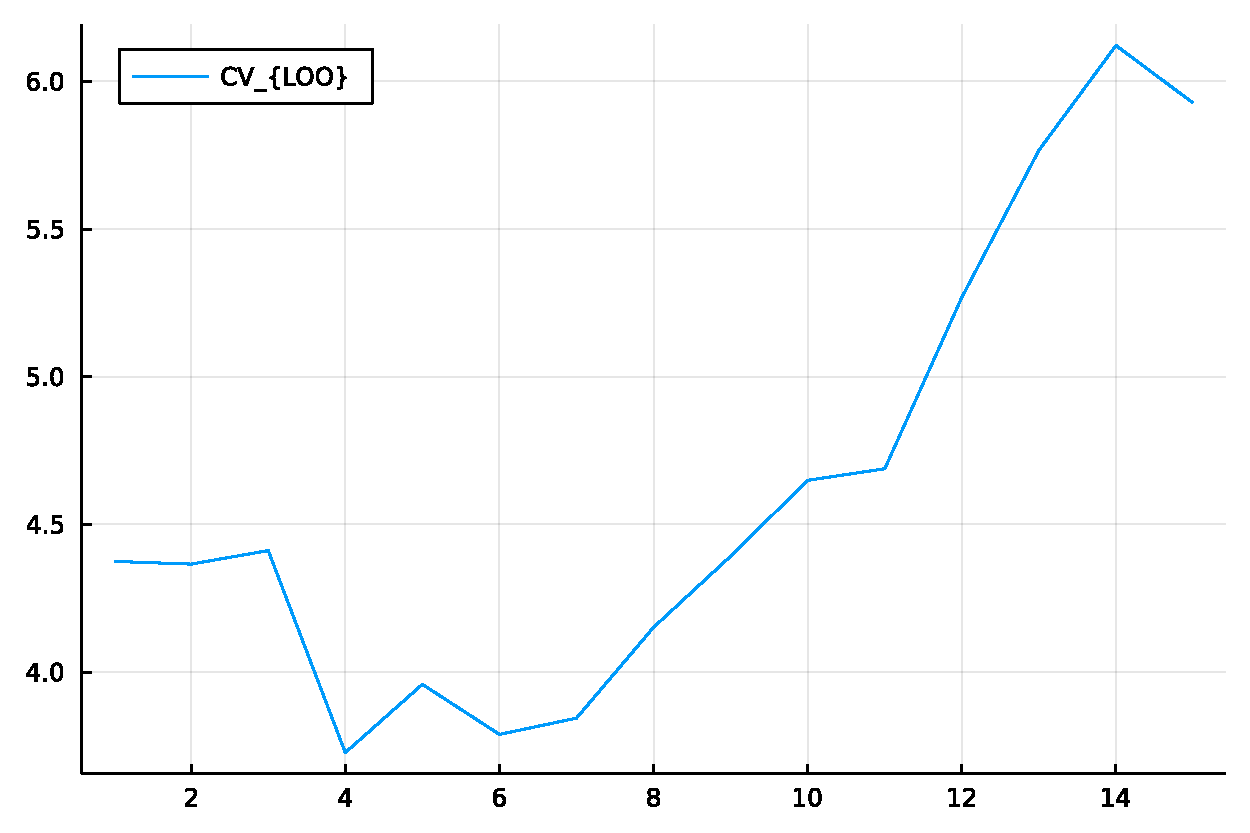
\includegraphics[width=.7\textwidth]{Result/CVLOO.pdf}
    \caption{$\mathrm{CV_{LOO}}$}
\end{figure}

図2より,knot数が4のときに最も値が小さくなっていることから4が最適であろうと考えた.

\section{}

多項式の場合は学習誤差は次の式で表されるため,データから計算可能なので単調に減少する.

\begin{equation}
\frac{1}{n} \sum_{i=1}^{n}\left(\hat{f}\left(\boldsymbol{x}_{i}\right)-y_{i}\right)^{2} , (\hat{f}(x)は学習データから推定された回帰係数)
\end{equation}

スプラインの場合は,次の式を小さくすることを目標にしているため,多項式回帰とは違い2乗誤差の値が単調にならない.
\[
\text { モデル: } \quad y_{i}=f\left(x_{i}\right)+\varepsilon_{i}, \quad \varepsilon_{i} \text { はノイズ }
\]
\begin{equation}
\sum_{i=1}^{n}\left(y_{i}-f\left(x_{i}\right)\right)^{2}
\end{equation}
\end{document}
